\newpage
\section{Statistical Model Checking}

When a model rely on stochastic behaviours, such as randomness, its state-space grows exponentially (sometimes called a state-space explosion) therefore an exhaustive search determining whether if some property holds is not possible in reasonable time. 
Instead one can estimate a percentage chance a property holds, within a given probability of uncertainty, with a Statistical Model Chcker (SMC). 

%UPPAAL SMC Explanation
\subsection{UPPAAL SMC}\label{subsec:uppaalsmc}
\begin{wrapfigure}[18]{r}{0.3\textwidth}
\centering
  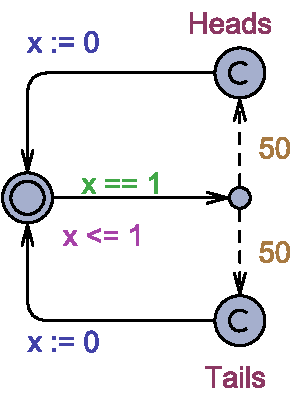
\includegraphics[width=0.3\textwidth]{Figures/Model/Simple_SMC.pdf} 
\caption{A simple UPPAAL SMC model with weighted edges. }
\label{fig:simpleSMC}
\end{wrapfigure}

To do this in UPPAAL there is an extension called UPPAAL SMC, a full tutorial is available here ``Uppaal SMC Tutorial''\cite{DBLP:journals/sttt/DavidLLMP15} by Alexandre David, Kim G. Larsen, Axel Legay, Marius Miku\v{c}ionis, Danny B\o gsted Poulsen.

In UPPAAL SMC there is a new type of edge, this is a weighted edge and is shown as a dashed line. 
An example of this can be seen in figure \myref{fig:simpleSMC}. 
The figure shows a simple UPPAAL SMC model, following the initial state there is a ``branch point'' from which there are two weighted edges.
The number by the weighted edges give their probability of being taken, this simple concept allows UPPAAL SMC to do randomness without having to explore the full state-space, as it can run simulations taking each edge a number of times corresponding to their weights. 
This example simulates a coin toss, giving 50 \% chance of heads and 50 \% chance of tails. 

UPPAAL SMC can additionally draw several types of plots which shows what the chance of a given query being true after a given run duration.

It is possible to set the statistical parameters for UPPAAL SMC, such as: Probability uncertainty, Probability of false negatives and Probability of false positives. 
Setting these parameters closer to zero will cause the time it takes to verify a query for a model to increase drastically, however it will also be more accurate. 

%Description of changes to the model in UPPAAL

\subsection*{Changes to the model}

The UPPAAL model shown in \myref{sec:themodel} has gone through extensive changes to accomodate the challenges posed of multiple devices starting at the same time.
The complete model can be seen in the back of the project report printed on a A3-paper, and it can also be found on the CD, which is also in the back of the project folder, however the code for the model can be found in \myref{UPPAAL-CCRC-Code}.


\paragraph{Jamming} can now occur since multiple devices are turned on at the same time, which means that more than one device is now able to transmit at the same time.
If two or more devices transmit at the same time, i.e. a jam, then none of the receiving devices will be able to receive any payloads, this is also mentioned in \myref[name]{subsubsec:RadioHead}, this needs to be modelled in UPPAAL. 
%When this happens, it has been mentioned in \myref[name]{subsubsec:RadioHead}, that nothing is detected by the receivers, therefore a mechanism making sure that when two devices are trying to transmit at the same time, nothing will be received by anyone are needed in UPPAAL. 

\paragraph{Multiple Startup.}
In the previous model presented in \myref[name]{sec:themodel} only one device was able to start at a time, as there was nothing to handle multiple starting at the same time.

\begin{wrapfigure}[21]{r}{0.5\textwidth}
    \centering
    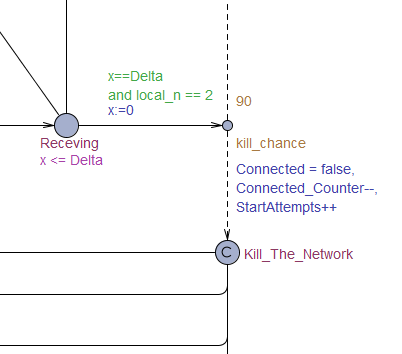
\includegraphics[width=0.5\textwidth]{Figures/Model/Screenshot_Of_Kill.png} 
    \caption{Graph showing the split node after not receiving, where there is a chance for the device to start over and kill the network.}
    \label{fig:Screenshot_Of_Kill}
\end{wrapfigure}

This limitation will be removed in this model.
To stop devices from being alone in a network forever, a split node is made when nothing is received in a time slot, where the device is alone in the network, i.e. the \texttt{local\_n} of the device is equal to 2.
This split node has 2 outgoing edges, one edge which has a probability weight of 90, which makes the device go back into its main loop, and another edge with a probability of \texttt{kill\_chance} (10 \%), which make the device kill the network, and start listening again.
When this happens the exponential backoff method is used, which means for each time a device kills the network it will have a chance of listening for a longer period of time, according to the specification in the previous sections.
This are the changes needed for the model, in order for the devices to start trying to connect to the same network instead of multiple networks.
\myref{fig:Screenshot_Of_Kill} shows the split node leaving the location after not receiving a transmission.


\paragraph{Multile Devices Connecting.}
The other problem is for when devices try to connect to the same network at the same time.
A verification loop has been created for the model, where all devices which transmitted that they wanted to join the network will listen for the number of devices acknowledging their request of joining the network.
If the amount of acknowledgments are lower than half of the devices in the network, they will also use the exponential backoff method, where they will wait for a random number of frames, in an increasingly larger range, with a cap of 31 frames (It only require one acknowledgment in the CCRC, but this solutions is chosen, to easier expand to CCUC).
This is the only change needed for handling multiple devices connecting to the network, the specifics of the implementation of this on the model will not be presented in this section, but for the curious reader the specifics can be seen in the back as previously mentioned.

%New Queries using SMC

\subsection*{Verifying using SMC}

Some of the queries presented in the previous UPPAAL section, \myref[name]{sec:verifyingTheModel}, make no sense for the new model, as now multiple networks should be running at the same time when the devices first start up, and therefore checking if the value of \texttt{i} is the same for all devices in a certain state makes no sense.
When verifying using SMC then the querys will yield a probability of being true within a given confidence interval, rather than true or false as in the normal UPPAAL.
Therefore the queries will all except for one be checking for the probability of them being true over time, when at least 3000 UPPAAL time units has passed.
The choice of 3000 time units is because this gives enough time for all devices to start up, and at least as some of them should have started a network. 
It should be noted that the model uses time estimates which roughly translate to the time being used in each phase for the hardware used in this project, where a time-slot length is $\delta = 250$.

All the queries have been run with five devices in the system, and a confidence of 0.999.
All queries' cumulative probability is shown on \myref{fig:ConnectQueryTime}.
The first query is the only query which was also used on the earlier model, and it will still give a result indicating the query holds.

\begin{lstlisting}[style=UPPAAL, title={This query requires that eventually if all devices are connected, then no pair of devices have the same \texttt{k}, unless the pair consists of the same two devices. This is true.}]
1. A<> forall(i : id_t) forall(j : id_t) Device(i).Connected and
         Device(j).Connected and Device(i).k == Device(j).k imply i == j
\end{lstlisting}

\begin{lstlisting}[style=UPPAAL, title={This query asks after 3000 UPPAAL time units has passed, what then is the probability that if two devices \texttt{i}, and \texttt{j} are connected to a network that their local values of \texttt{n} are the same, and that they are both connected to the same network. This means that the devices are connected to the same network. UPPAAL runs this query and within 3451 runs [0.998,1] with confidence 99.9 \% this is true. }]
2. Pr[<=300000] ( <> forall(i : id_t) forall(j : id_t) (time > 3000) 
    and (Device(i).Connected and Device(j).Connected 
    imply ((Device(i).local_n == Device(j).local_n)
        and Device(i).local_network_id == Device(j).local_network_id)))     
\end{lstlisting}

\begin{lstlisting}[style=UPPAAL, title={This query asks after 3000 UPPAAL time units has passed, what then is the probability that if a device \texttt{i} and a device \texttt{j} is both connected that then \texttt{i}'s values of \texttt{k} will be larger than zero and smaller than any \texttt{n}, and that they are connected to the same network. This query insures that all the \texttt{k}-values are within the wanted range after a network is made. UPPAAL runs this query and within 3451 runs [0.998,1] with confidence 99.9 \% this is true.}.]
3. Pr[<=300000] ( <> forall(i : id_t) forall(j : id_t) (time > 3000) 
    and (Device(i).Connected and Device(j).Connected 
    imply (Device(i).k < Device(j).local_n and Device(i).k > 0) 
        and Device(i).local_network_id == Device(j).local_network_id))

\end{lstlisting}

\begin{lstlisting}[style=UPPAAL, title={This query asks after 3000 UPPAAL time units has passed, what then is the probability that a device \texttt{i} has a local value of \texttt{n} to be equal to the number of devices plus the the empty slot, which is \texttt{N} + 1, which means that all devices are in the same network. UPPAAL runs this query and within 3451 runs [0.998,1] with confidence 99.9 \% this is true.}]
4. Pr[<=300000] Pr[<=300000] ( <>  forall(i : id_t) (time >3000) 
    and Device(i).local_n == N + 1)
\end{lstlisting}

\begin{lstlisting}[style=UPPAAL, title={This query is a generalisation of the previous which includes a check of whether when one device finish transmitting then the rest are just finished receiving. UPPAAL runs this query and within 3451 runs [0.998,1] with confidence 99.9 \% this is true.}]
5. Pr[<=300000] ( <>  forall(i : id_t) forall(j : id_t) (time >3000) 
    and (Device(i).local_n == N+1) 
    and (Device(i).Done_Transmitting 
    imply (Device(j).Just_Received or i==j)))
\end{lstlisting}

\myref{fig:ConnectQueryTime} shows a graph of all the queries.
As can be seen the change in probability for the new model approaches one as time increases, and appears to be a logarithmic growth.
So according to UPPAAL the new model will eventually connect all the devices, however it might take some time for it to do so.
In the worst case the random numbers generated will keep causing collisions\todo{Skriver vi collisions eller jam, generelt?  - Troels}, however this happening is very unlikely. 
There are many possible explanations\todo{Hvilke og hvorfor? - Troels} for what causes the longer runs, but it it important to note that, the longer the devices are running the greater the probability is of establishing a stable network.

\begin{figure}[ht]
  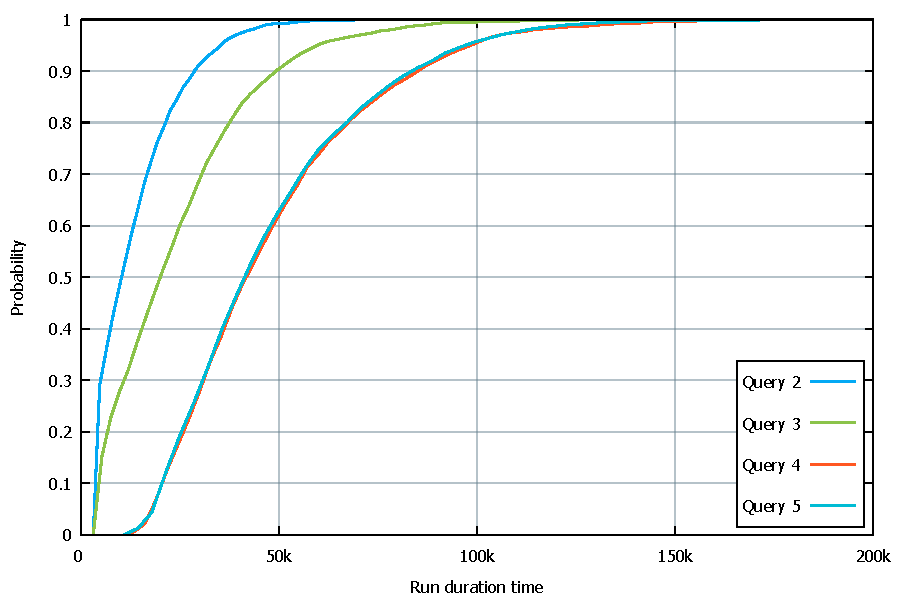
\includegraphics[width=1\textwidth]{Figures/Graphs/gnuplot/uppaal/graph.pdf} 
\caption{Graph of the UPPAAL SMC queries, in which the cumulative probability increase over time.}
\label{fig:ConnectQueryTime}
\end{figure}

\bigskip
A comparison has been made for this model with the previous model in \myref{sec:themodel}, while allowing the devices to start at the same time.
Query 4 can be run on both models, but on the older simpler model it will, when run with five devices, yield the result [0.0, 0.019], which means that it will probably never succeed.
So a change to the models allow the devices to leave the initial location at any moment between 0 and 30000 UPPAAL time units, and different results occur; the devices will now sometimes have enough interval between activation so that a stable network will be created. 
The probability result is [0.75,0.77].
Therefore this shows that if the devices are started with an interval in the old model, there still is a reasonable success rate, but as soon as they start at the same time, it doesn't work. 

The changes are the same for both models and can be seen on \myref{lst:startuptimeChanceListing}. \todo{Denne myref referer til en listing som var den en section. ??? - Troels}


\begin{lstlisting}[style=UPPAAL, title={Change in the start up time for devices.}, label={lst:startuptimeChanceListing}]
//Original
int Startup_Time = Initial_Wait_Time*2;

//Change
int Startup_Time = Initial_Wait_Time*20;
\end{lstlisting}


The old model performs significantly worse that the new one, and will not always reach a stable correctly created network, and this is as mentioned only possible whenever there is a interval between activation of the devices.

The changes in the new model which handles that devices start at the same time also improves, in sense of speed, from the fact that they may start with bigger intervals, the results of running the query can be seen on \myref{CompareGraph}. \todo{Hvad menes der med denne sætning? - Troels}
Changing the new model's startup time is done so the two models can be compared in speed as-well as probability of creating a stable network under the same circumstances.

\begin{figure}[ht]
  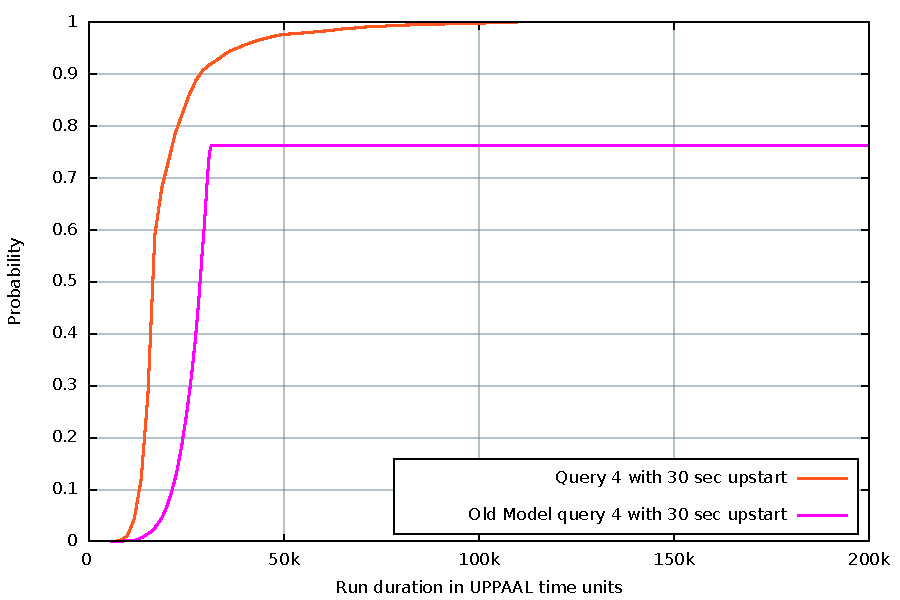
\includegraphics[width=1\textwidth]{Figures/Graphs/gnuplot/uppaal_Compare/graph.pdf} 
\caption{Graph of the query number 4, for both the old and the new model so their successrate and speed can be compared.}
\label{CompareGraph}
\end{figure}


\section{Conclusion}
This chapter presented a way to handle the startup of multiple devices, which made use of the method exponential backoff, which results in an increasingly randomly generated number of wait time for the devices. 
The randomness results in all devices eventually becoming connected to the network since they will be split up and thus stop jamming each other.
The UPPAAL model created data, which can be seen on \myref{fig:ConnectQueryTime}.
The data shows that the Arduinos will eventually be connected to the same network, however it does take some time, approximately $150 000$ UPPAAL time units.
This means that an implementation of this design should be able to solve the issues of turning on more Arduinos at the same time, assuming our assumptions are correct.
